\chapter{Example accident model}
\label{ch:accident_model}
Using FRAM retrospectively will, hopefully, identify some of the critically constrained couplings between functions in a system. Applying this knowledge, it will be possible not only to build safer, but also more resilient system.\\
\\
This chapter will take a relevant near-miss and model it with the procedure suggested by FRAM. 

\section{Near miss at Train crossing}
Modelling a near miss incident is not very common, though very rewarding in terms of drawing experience from them. A more elaborate explanation of what a near miss is, see section \ref{sec:near_miss}

%Previous studies\cite{belmonte2011interdisciplinary}

\subsection{Background}
At Grenåbanen on tuesday the 26th of March 2010, at 14:40, an ambulance was intentionally led over railway crossing that should have been secured. This situation led to a near-miss, and luckily no one was harmed.

\subsubsection{Official accident report}
Train RV 4940 in transit from Grenå towards Aarhus was signalled that crossing 128a was secured.

Shortly after, the train driver realized that 2 railway employees were located on the track. The driver did not do anything further as he assumed they would move when they saw the train.

As the train approached the crossing, an ambulance with siren signal entered the crossing - from the road side. The train driver used the emergency brake, hereby avoiding collision with the ambulance. According the the train driver, the collision was imminent.\\
\\
The 2 railway employees reported that, they though they would be able to assist the ambulance in reaching its destination faster, by leading it into the crossing before the train arrived, by misjudged the situation.\\
\\
The document ``udrykningsbekendtgørelsen'' (the official notice regarding emergency) states that the driver of an emergency vehicle, must at all times abide signals or other instructions, at railway crossings

Following the initial investigations and evaluations of the data available - the accident investigation committee reached the following conclusion; further studies would not necessarily lead to preventative recommendations, or result in findings leading to significant improvements in railway safety.

With reference to Danish railway legislation, the accident investigation committee decided not to perform further studies. 

\subsection{Assumptions}
As there are only crossing bars in the driving direction - it is assumed that the crossing bars were in place as the event took place. Figure \ref{fig:ambulance_path} illustrates the assumed path of the ambulance and the placement of the crossing bars.
\begin{figure}
 \centering
   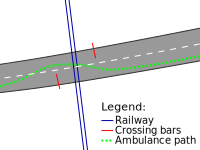
\includegraphics[width=150pt]{figures/accident_overview.pdf}
 \caption{Assumed ambulance path (train approaching from the north)}
 \label{fig:ambulance_path}
\end{figure}
The path taken by the ambulance indicates that it had to slow down, maybe even significantly. This adds to the total variability of the pseudo-barrier which here is time.

\subsubsection{FRAM model}
TODO
%It is assumed that the two employees manually secured the tracks


% 1. Define the purpose of the analysis: The purpose here is to look at what happended and discuss the variability of the system in total

% 2. Identify and describe the relevant system functions.

% 

Functions: 
Signal

(Crossing bar)


\subsubsection{Functions}
It is assumed that the two employees manually initiated the securing of the crossing. The function/activity is represented in table \ref{table:function_initiate_securing}. To initiate the securing, the car drivers must first be notified of the pending closing of crossing bars. This must be done some time prior to the train arrival, as response time on clearing is relativity high.
\begin{table}[h]
\centering
    \begin{tabular}{ | l | r | }
    \hline
    Function     &  Initiate securing of crossing\\ \hline \hline
    Input        &  \\ \hline
    Output       &  Signal the car drivers\\ \hline
    Precondition &  Incoming train\\ \hline
    Resource     &  \\ \hline
    Time         &  Safe time before train arrives\\ \hline
    Control      &  Regulations\\ \hline
    \end{tabular}
\caption{FRAM table of the initiating activity}
\label{table:function_initiate_securing}
\end{table}

When the road side is cleared, the crossing bars are lowered - effectively blocking it. It is essential that the cars have left the crossing. This function is modelled in table \ref{table:function_block_from_road_side}.

\begin{table}[h]
\centering
    \begin{tabular}{ | l | r | }
    \hline
    Function     &  Block passage from road side\\ \hline \hline
    Input        &  Signal the car drivers\\ \hline
    Output       &  Lower the crossing bars\\ \hline
    Precondition &  \\ \hline
    Resource     &  \\ \hline
    Time         &  Time sufficient to clear crossing\\ \hline
    Control      &  \\ \hline
    \end{tabular}
\caption{FRAM table of the blocking function}
\label{table:function_block_from_road_side}
\end{table}

Table \ref{table:function_allow_passage_from_train_side} models the function that allows train passage. As the crossing is interlocked, it must be secured for train passage before the train will be able to enter it. This is usually enforced by both a signal, and ATC (\ref{sec:atc}).

\begin{table}[h]
\centering
    \begin{tabular}{ | l | r | }
    \hline
    Function     &  Allow passage from train side \\ \hline \hline
    Input        &  Train has enters crossing\\ \hline
    Output       &  Train has left crossing\\ \hline
    Precondition &  Crossing bars lowered\\ \hline
    Resource     &  \\ \hline
    Time         &  Must pass within blocking-time window\\ \hline
    Control      &  ATC\\ \hline
    \end{tabular}
\caption{FRAM table representing the activity of allowing train passage}
\label{table:function_allow_passage_from_train_side}
\end{table}
When the train has passed, the crossing will be able to unblock the road side after a safety delay. Some crossings will automatically open after a timeout has occurred, even if no train has passed - of course while blocking the railway. Table \ref{table:function_unblock_road_side}.
\begin{table}[h]
\centering
    \begin{tabular}{ | l | r | }
    \hline
    Function     &  Unblock road side \\ \hline \hline
    Input        &  Train has left crossing\\ \hline
    Output       &  Unblock road side passage\\ \hline
    Precondition &  \\ \hline
    Resource     &  \\ \hline
    Time         &  Safety delay\\ \hline
    Control      &  Timeout\\ \hline
    \end{tabular}
\caption{FRAM table representing the function of unblocking the road side}
\label{table:function_unblock_road_side}
\end{table}

\begin{figure}[h]
 \centering
   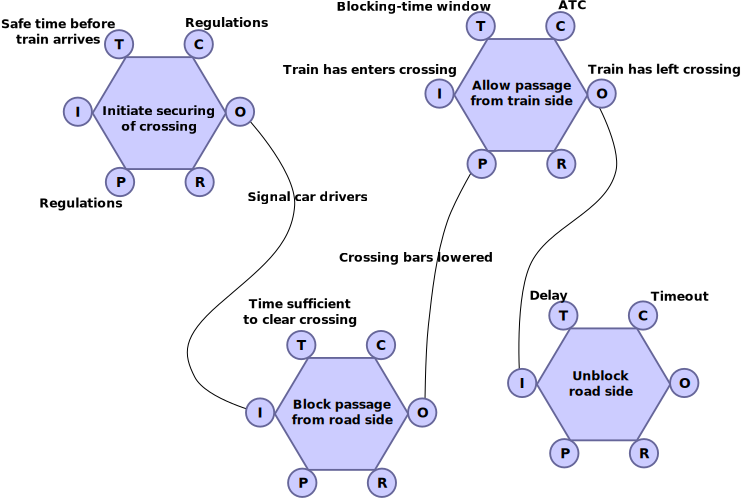
\includegraphics[width=1\textwidth]{figures/Accident_fram_model.pdf}
 \caption{Graphical FRAM representation}
 \label{fig:fram_graphical}
\end{figure}

This graphical representation shows quite clearly that time is an essential aspect of every activity and function - hence every small variability in a function will resonate and propagate onto the next.

\subsection{Barriers}
There are a number of barriers in place here:
\begin{itemize}
  \item A physical barrier that is intercoupled with a incorporeal barrier; the crossing bars that depend on driving in the right side of the road (following traffic laws).
  \item Time - the essential barrier. Safety functions depend largely on having the time to complete their cycle.
  \item Two incorporeal barriers; ``udrykningsbekendtgørelsen'' and the railway legislation.

\end{itemize}

\section{Discussion}
%TODO In general, like in statistics, Corrolation does not imply causation.

The near-miss her is beyond the scope of the intended operation/design of ATC(\ref{sec:atc}) and is a perfect example of high variability in a system. Everything works as intended, until the railway workers are affected by a disturbance that ultimately leads to two time constraint pressures; one from the Ambulance, and one from the approaching train.

On the remedial side, there could be a gain by adding a second set of crossing bars, meaning that both driving lanes of the road will be blocked. This will prevent this barrier to be overridden entirely. Adding a second set of bars would introduce the hazard of ``trapping'' cars inside the secured crossing, but could be avoided by delaying the lowering of the second set of bars for a short time after the first set.

%TODO The fields usabilty engineering and safety enginering are closely related in terms of clear communication.

\chapter{Conclusion}
